\documentclass{standalone}

\usepackage{circuitikz}

\begin{document}

% INT_AY20_MP2_L29_Fig01-Attracting_masses.png

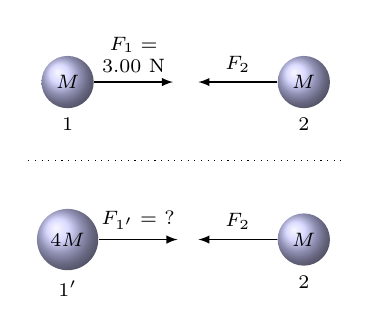
\begin{tikzpicture}[> = latex, font = \scriptsize]

	% Initial picture
	
		% Masses
		
		\node (close1) [circle, ball color = blue!20, label = {below : 1}] at (-1.5, 1) {$M$};
		\node (close2) [circle, ball color = blue!20, label = {below : 2}] at (1.5, 1) {$M$};
		
		% Vectors for forces
		
		\begin{scope}[->]
		
			\draw (close1.east) -- node [midway, above, align = center] {$F_1 =$\\3.00 N} ++ (1, 0);
			\draw (close2.west) -- node [midway, above] {$F_2$} ++ (-1, 0);
		
		\end{scope}
		
	% Separator line
	
	\draw [dotted] (-2, 0) -- (2, 0);
	
	% Final picture
		
		% Masses
		
		\node (close1) [circle, ball color = blue!20, label = {below : 1$^\prime$}] at (-1.5, -1) {$4M$};
		\node (close2) [circle, ball color = blue!20, label = {below : 2}] at (1.5, -1) {$M$};
		
		% Vectors for forces
		
		\begin{scope}[->]
		
			\draw (close1.east) -- node [midway, above] {$F_{1^\prime} = $ ?} ++ (1, 0);
			\draw (close2.west) -- node [midway, above] {$F_2$} ++ (-1, 0);
		
		\end{scope}

\end{tikzpicture}

\end{document}